\section{HomeScreen}

Der Home-Screen bildet die zentrale Interaktionsebene zwischen dem Nutzer und Sokka.

Er wird aus einem \lstinline{DefaultTabController}-Widget aufgebaut und besteht aus vier
verschiedenen Tabs, die per Swipe gewechselt werden können und die Parent-Elemente
für alle Views bilden.

Für die Navigation zwischen den Views des Home-Screens wird ein \lstinline{TabBar}-Widget
benötigt, welches dem \lstinline{bottomNavigationBar}-Property übergeben werden muss.

Mithilfe einer solchen Tab-Bar kann neben einer Beschriftung inklusive Icon
der einzelnen Tabs auch ein Indicator eingebaut werden, der anzeigt, auf welchem Tab (und damit View)
sich der Nutzer gerade befindet.

\begin{code}[h]
    \centering
    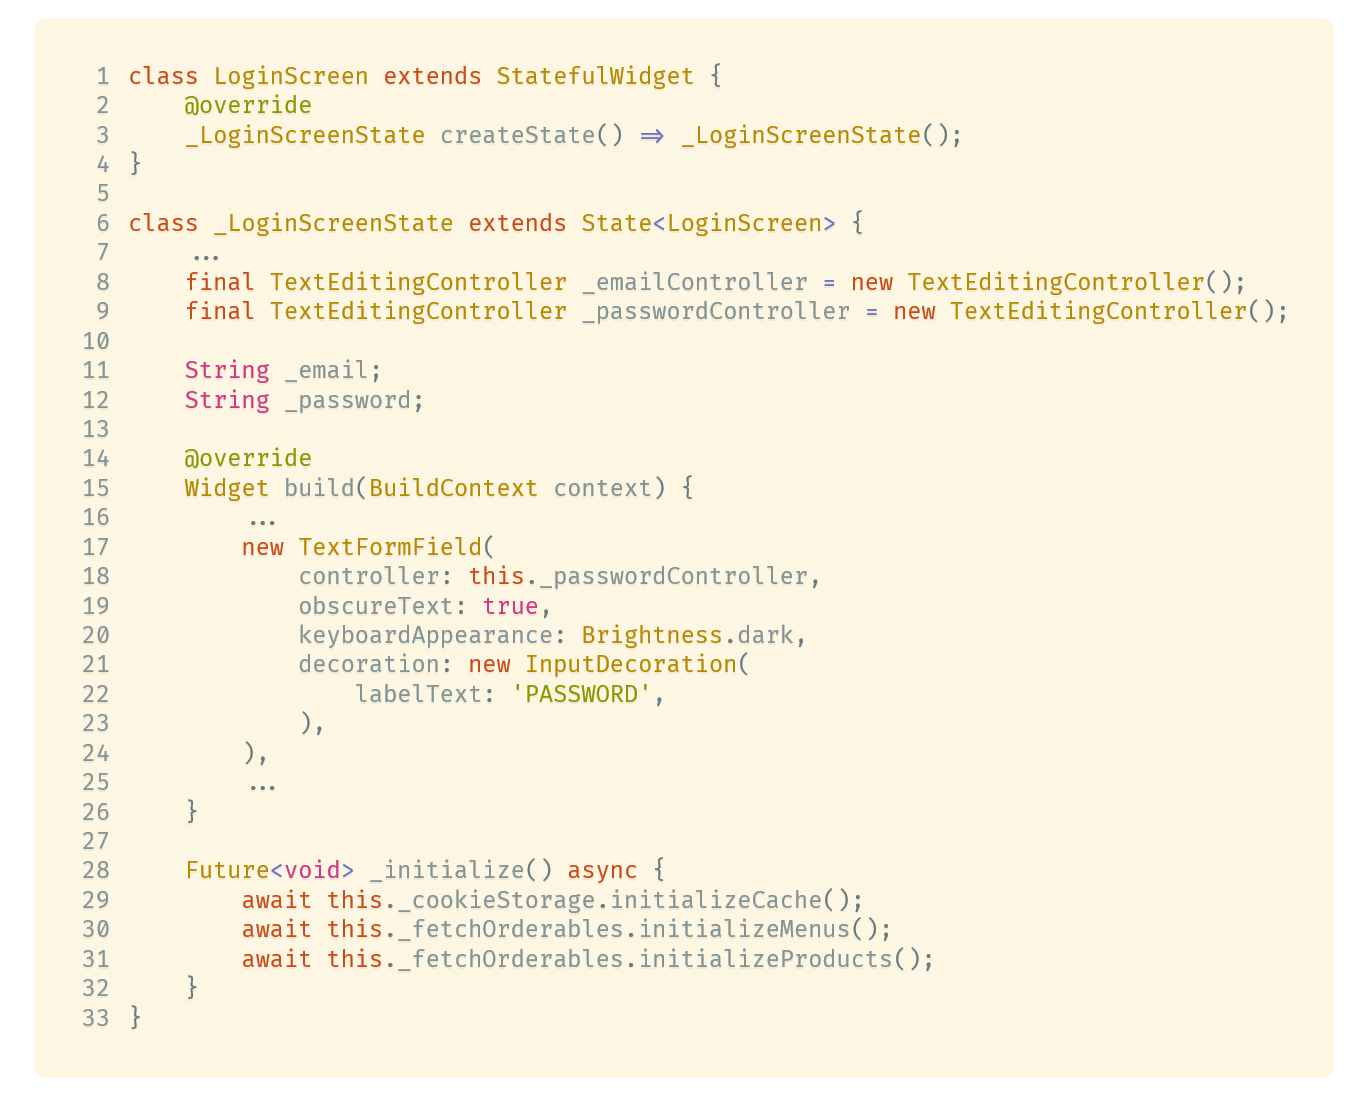
\includegraphics[width=1\textwidth]{images/Client/screens/home/tabbar.png}
    \caption{DefaultTabController mit vier Tabs und Tab-Bar zur Navigation}
\end{code}